%===============================================================================
% DOCUMENT
%===============================================================================

%% Document class
\documentclass[a4paper,12pt]{scrreprt}

%% Include packages
\usepackage{packages}
\usepackage{float}

\begin{document}

%% Include custom commands
\include{commands}

\pagenumbering{gobble}

%% Build cover
\definecolor{titlepagecolor}{RGB}{245,130,32}

%==========================================================================
% COLORED BAR ON THE LEFT SIDE
%==========================================================================

\backgroundsetup{
    scale=1,
    angle=0,
    opacity=1,
    contents={
        \begin{tikzpicture}[remember picture,overlay]
            \path [fill=titlepagecolor] (-10.5,-15) rectangle ++ (5,30);
            \node[color=white] at (-6.60,-11.5) {\bfseries {\fontsize{120}{60} \textsf{I}}};
            \node[color=titlepagecolor] at (-4.20,-11.5) {\bfseries {\fontsize{120}{60} \textsf{A}}};
        \end{tikzpicture}
    }
}

%==========================================================================
% COVER PAGE CONTENT
%==========================================================================

\title{\LARGE{Otimização de Distribuição Alimentar numa Catástrofe}}

\author{
    Flávia Alexandra da Silva Araújo (A96587)\\ \quad
    Joshua David Amaral Moreira (A105684)\\ \quad
    Miguel Fernandes Barbosa (A104451)\\ \quad
    Miguel Torres Carvalho (A95485)\\ \quad
}

%% Date
\date{\today}

%% Course
\newcommand{\Course}{Licenciatura em Engenharia Informática}

%% Department
\newcommand{\Department}{Escola de Engenharia}

%% UniName
\newcommand{\UniName}{Universidade do Minho}

%% UniPic
\newcommand{\UniPic}{
\includegraphics[width=120pt]{img/eeum.png}}

%% University
\newcommand{\University}{
    \begin{flushleft}
         \UniPic   
    \end{flushleft}
    \textcolor{gray}{\small\textbf{\textsf{\UniName}}}\par
    \textcolor{gray!80!white}{\small{\textsf{\Department}}}\par
    \textcolor{gray!70!white}{\small{\textsf{\Course}}}
}

%% UC
\newcommand{\UC}{
    \begin{flushleft}
        \par\textcolor{titlepagecolor}{\Large\textbf{\textsf{Inteligência Artificial}}}
    \end{flushleft}
}

%% Project Phase
\newcommand{\SubTitle}{
    \begin{flushleft}
        \large\textbf{Resolução de Problemas com Algoritmos de Procura}
    \end{flushleft}
}

%% Group Info
\newcommand{\GroupInfo}{\par Grupo 21}

%% GitHub Repo
\newcommand{\GitHubRepo}{\par\url{https://github.com/flaviaraujo/project-IA}}

%% School Year
\newcommand{\SchoolYear}{
    \par\small{\textsf{Ano Letivo de 2024/2025}}
}

%% Define new command to show title, author and date
\makeatletter
\let\Title\@title
\let\Author\@author
\let\Date\@date
\makeatother

%==========================================================================
% BEGIN COVER PAGE
%==========================================================================

%% Make cover page
\newcommand{\makecover}{

%% Removes page number on footer
\thispagestyle{empty}

%% No indentation
\setlength{\parindent}{0em}

%% Put Background defined on \backgroundsetup, in this page
\BgThispage

%% Changing geometry to prevent overlay with text
%% At the end of back cover, geometry is default with \restoregeometry
\newgeometry{top=4cm,left=6cm,right=2cm,bottom=2cm}

%% builds university info defined previously
\University
\vspace{1cm}
\UC
\SubTitle
\SchoolYear

\vspace*{4cm}
%% bigger space (i think its the default one) between paragraphs
\setlength{\parskip}{1em}

%% builds title info defined previously
\par\textbf{\textsf{\huge\Title}}
\vspace{1cm}
%% builds author(s) info defined previously
\par\Author

\vspace{0.5cm}

%% builds date info defined previously
\par\Date
\restoregeometry
\pagebreak

}

%==========================================================================
% END COVER PAGE
%==========================================================================

\makecover

%% Default geometry
\newgeometry{top=3cm,left=3cm,right=3cm,bottom=4cm}

%% Save default geometry
\savegeometry{default}

%% Load default geometry with:
% \loadgeometry{default}


%===============================================================================
% BEGIN ABSTRACT PAGE
%===============================================================================

\renewenvironment{abstract}
 {\par\noindent\textbf{\Large\abstractname}\par\bigskip}
 {}

\begin{flushleft}
\begin{abstract}
    As catástrofes naturais, como furacões, terremotos e inundações, frequentemente deixam um rasto
    de destruição, tornando fundamental a gestão eficiente de recursos para mitigar o impacto humanitário.
    Em situações de emergência, otimizar a distribuição de suprimentos essenciais, como alimentos, água e
    medicamentos, pode ser a diferença entre salvar ou perder vidas.

    Este trabalho propõe uma abordagem baseada em inteligência artificial, especificamente através de algoritmos
    de procura, para resolver o problema de logística em cenários de crise. A formulação do problema considera
    fatores como a perecibilidade dos alimentos, as limitações operacionais dos veículos, e a urgência das necessidades
    das áreas afetadas. O objetivo principal é minimizar o tempo de resposta, reduzindo desperdícios e maximizando a
    eficiência operacional.

    Além disso, este estudo explora os diferentes resultados obtidos por diversos algoritmos de procura, bem como as
    diferentes definições de heurísticas influenciam os mesmos.
    Com uma análise focada na eficiência logística, tanto a nível de recursos utilizados como tempo de resposta.
    
    \par \textbf{Área de Aplicação}: Inteligência Artificial, Distribuição de Recursos.
    \par \textbf{Palavras-Chave}: Algoritmos de Procura, Heurísticas, A*, Gulosa, BFS, DFS, Procura Uniforme.
\end{abstract}
\end{flushleft}

\pagebreak

%===============================================================================
% END ABSTRACT PAGE
%===============================================================================


%===============================================================================
% BEGIN INDEXES PAGES
%===============================================================================

%% Changes table of content name
\renewcommand{\contentsname}{Índice}
\renewcommand{\listfigurename}{Índice de Figuras}
\renewcommand{\listtablename}{Índice de Tabelas}

\tableofcontents
\pagebreak

\listoffigures
\pagebreak

\listoftables
\pagebreak


%===============================================================================
% END INDEXES PAGES
%===============================================================================

\pagenumbering{arabic}

%===============================================================================
% BEGIN DESCRIÇÃO DO PROBLEMA
%===============================================================================

\chapter{Descrição do Problema}

Este problema trata-se de um cenário de gestão de recursos em situações de emergência, onde é 
necessário coordenar a distribuição de suprimentos em zonas afetadas por desastres naturais.
O objetivo é otimizar a distribuição de recursos, minimizando o tempo de resposta e garantindo a
satisfação das necessidades das zonas afetadas.

O problema é composto por um conjunto de localizações, algumas das quais são zonas afetadas (e, de entre
estas, algumas com maior urgência), com diferentes níveis de acesso. Para chegar a estas zonas, é necessário utilizar veículos que partem
de diferentes localizações. Existem diferentes tipos de veículos: mota, carro, camião, \textit{drone}, helicóptero,
avião, e barco. Cada veículo tem uma capacidade de carga, velocidade, capacidade de combustível e gasto de combustível
diferente. Como tal, deve ser feita uma gestão eficiente dos mesmos, de forma a que sejam utilizados de maneira
a otimizar as suas capacidades de transporte.

\begin{table}[ht]
    \centering
    \small % Reduce font size
    \setlength{\tabcolsep}{0.5pt} % Adjust column spacing
    \renewcommand{\arraystretch}{1.2} % Adjust row spacing
    \fontsize{9}{10}\selectfont
    \begin{tabular}{|c|c|c|c|c|c|}
        \hline
        \textbf{Veículo} & \textbf{Tipo} & \textbf{Capacidade (kg)} & \textbf{Velocidade (km/h)} & \textbf{Cap. Comb. (L)} & \textbf{Cons. Comb. (L/100km)} \\
        \hline
        Mota & Terrestre & 10 & 120 & 15 & 4 \\
        Carro & Terrestre & 500 & 160 & 50 & 8 \\
        Camião & Terrestre & 2000 & 100 & 300 & 30 \\
        \hline
        Drone & Aéreo & 5 & 100 & 5 & 2 \\
        Helicóptero & Aéreo & 700 & 250 & 300 & 70 \\
        Avião & Aéreo & 800 & 250 & 200 & 40 \\
        \hline
        Barco & Marítimo & 5000 & 50 & 1000 & 50 \\
        \hline
    \end{tabular}
    \caption{Características dos Veículos}
    \label{tab:veiculos}
\end{table}

Os suprimentos a distribuir são de diferentes tipos: alimentos, água e \textit{kits} de primeiros socorros. Cada zona afetada
tem necessidades específicas, que devem ser satisfeitas com a distribuição dos suprimentos. A distribuição dos suprimentos
deve ser feita de forma a minimizar o tempo de resposta e o uso de combustível, garantindo que as zonas com maior urgência
são atendidas primeiro, bem como minimizar o desperdício de suprimentos perecíveis.

%===============================================================================
% END DESCRIÇÃO DO PROBLEMA
%===============================================================================

%===============================================================================
% BEGIN FORMULAÇÃO DO PROBLEMA
%===============================================================================

\chapter{Formulação do Problema}

\begin{itemize}
    \item\textbf{Tipo:} Problema de Procura de Múltiplos Estados
    \item\textbf{Estado Inicial:}  Conjunto de nodos com suprimentos para distribuir.
    Zonas afetadas (catástrofes) com respetivas necessidades, e veículo(s) inicialmente estacionados, por um ou mais nodos, com combustível cheio e
    carga vazia.
    \item\textbf{Estado Objetivo:} Todas as zonas afetadas atendidas, com suprimentos distribuídos de
    forma eficiente, minimizando desperdícios de suprimentos perecíveis e combustível, assim como o tempo de resposta.
        \item\textbf{Operadores (Ações Disponíveis):} 
        \begin{itemize}
                \item\textit{Mover Veículo:} Deslocar um veículo de uma zona para outra, respeitando as limitações de combustível e condições da rota.
                \item \textit{Carregar Suprimentos:} Carregar suprimentos no veículo, respeitando a capacidade de carga do veículo.
                \item\textit{Descarregar Suprimentos:} Descarregar suprimentos existentes do veículo.
                \item\textit{Reabastecer Combustível:} Realizar paragens no percurso para reabastecimento dos veículos, tendo em conta o tempo
                necessário e as capacidades de combustível, tanto no nodo, como no veículo. 
        \end{itemize}
    \item\textbf{Custo da Solução:} O custo é calculado com base no tempo de resposta, combustível utilizado, e suprimentos distribuídos.
    \end{itemize}

%===============================================================================
% END FORMULAÇÃO DO PROBLEMA
%===============================================================================

%===============================================================================
% BEGIN USAGEM 
%===============================================================================
\newgeometry{top=2cm,left=3cm,right=3cm,bottom=3cm}

\chapter{Usagem}

O programa é executado através de \texttt{src/main.py}.
O programa aceita o argumento \texttt{--verbose} para mostrar informação detalhada dos algoritmos de pesquisa,
o que pode ser desativado ou ativado no menu principal.

Ao executar o programa, é apresentado um menu principal, onde o utilizador pode escolher entre diferentes opções:
\begin{figure}[H]
    \centering
    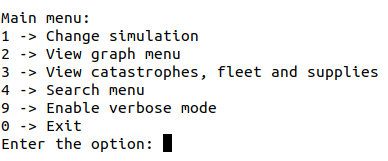
\includegraphics[width=0.55\textwidth]{img/main_menu.png}
    \caption{Menu Principal}
    \label{fig:menu}
\end{figure}

Caso o utilizador escolha a opção 1, é apresentado um menu para escolher a simulação a utilizar:

\begin{figure}[H]
    \centering
    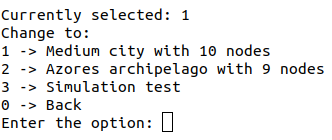
\includegraphics[width=0.5\textwidth]{img/change_simulation.png}
    \caption{Submenu de Simulações}
    \label{fig:change_simulation}
\end{figure}

\clearpage

Caso o utilizador escolha a opção 2, é apresentado o menu de visualização do grafo.
Neste, é possível imprimir o grafo, assim como nodos, arestas e valores heurísticos, de forma textual, bem como
é dada a opção de visualizar o grafo em formato de imagem, recorrendo à biblioteca \texttt{graphviz}, 
ou \texttt{matplotlib}.

\begin{figure}[H]
    \centering
    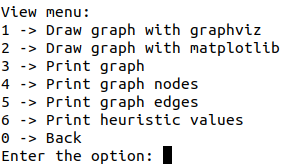
\includegraphics[width=0.5\textwidth]{img/graph_menu.png}
    \caption{Submenu Gráfico}
    \label{fig:graph_menu}
\end{figure}

Caso o utilizador escolha a opção 3, é apresentado em formato \textit{JSON} a lista de catástrofes, frota de veículos,
e suprimentos, com os detalhes respetivos de cada um.

\clearpage

Caso o utilizador escolha a opção 4, é apresentado o menu de algoritmos de procura, onde é possível executar
os algoritmos disponíveis: BFS, DFS, UCS, A* e Gulosa. Também é possível escolher a heurística a utilizar para algoritmos
de procura informada.

\begin{figure}[H]
    \centering
    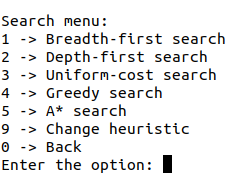
\includegraphics[width=0.4\textwidth]{img/search_menu.png}
    \caption{Submenu de Algoritmos de Procura}
    \label{fig:search_menu}
\end{figure}

\begin{figure}[H]
    \centering
    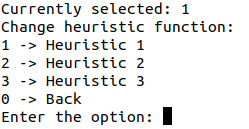
\includegraphics[width=0.4\textwidth]{img/change_heuristic.png}
    \caption{Submenu de Heurísticas}
    \label{fig:change_heuristic}
\end{figure}

Caso o utilizador escolha a opção 9, alterna o modo verboso, que, como supramencionado,
informação detalhada dos algoritmos de pesquisa, como o conjunto de veículos que conseguem aceder
a uma catástrofe a tempo, bem como os veículos designados para cada catástrofe.

A opção 0 permite terminar a execução do programa.

%================================================================================
% END USAGEM
%===============================================================================

%===============================================================================
% BEGIN TAREFAS REALIZADAS E DECISÕES TOMADAS
%===============================================================================
\chapter{Tarefas Realizadas e Decisões Tomadas}

\section{Grafos Criados}

O grafo correspondente ao problema é composto por um conjunto de vértices, que representam as localizações, e um conjunto de arestas,
que representam as ligações entre essas. Cada aresta tem a respetiva distância, o tipo desta ligação, o nível de acessibilidade, 
e uma percentagem de multiplicador de velocidade.
Na representação gráfica com a biblioteca \texttt{graphviz}, as arestas podem ter diferentes cores - azul para ligações marítimas, 
verde para ligações terrestres, e vermelho para ligações aéreas -,
bem como diferentes espessuras, que representam o nível de acessibilidade entre as localizações - quanto mais espessa a aresta, mais
tipos de veículos podem circular por ela. Por exemplo, uma aresta fina só pode ser percorrida por veículos ligeiros, como motas,
\textit{drones}, ou barcos pequenos, dependendo do método de viagem dessa aresta.

Foram efetuados os seguintes grafos para representar o problema:

\begin{figure}[H]
    \centering
    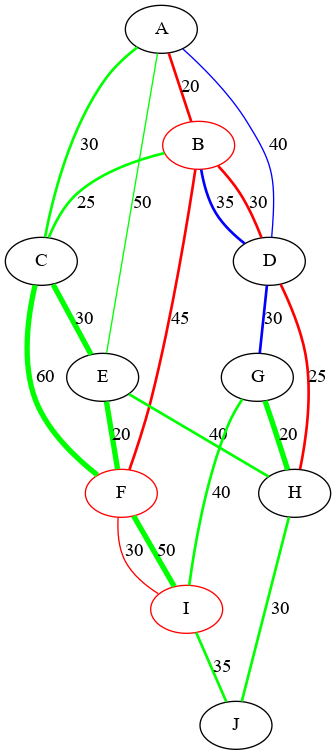
\includegraphics[width=0.3\textwidth]{img/graph_medium_city.png}
    \caption{Grafo de Simulação de uma Cidade Média}
    \label{fig:graph_medium_city}
\end{figure}

\begin{figure}[H]
    \centering
    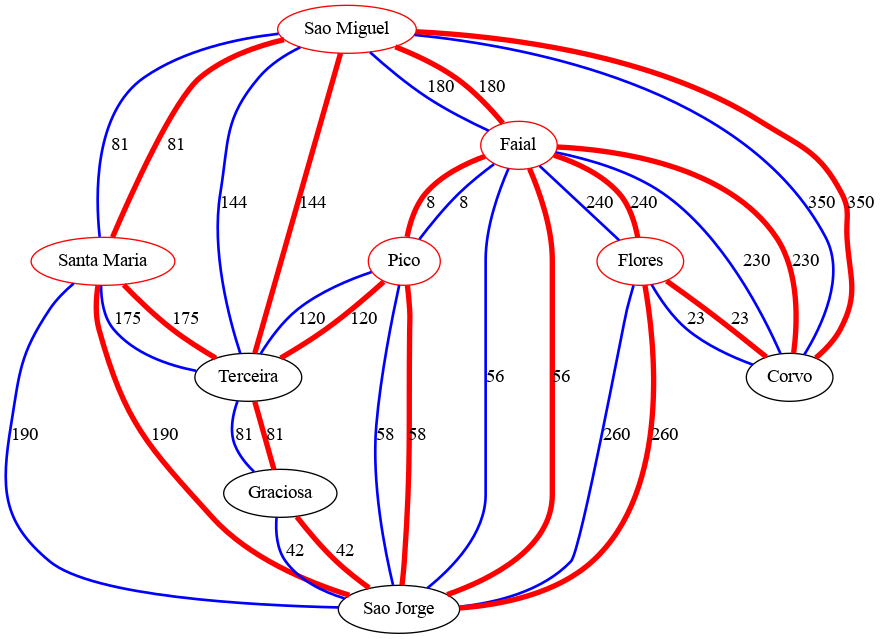
\includegraphics[width=0.85\textwidth]{img/graph_azores.png}
    \caption{Grafo de Simulação do Arquipélago dos Açores}
    \label{fig:graph_azores}
\end{figure}

\begin{figure}[H]
    \centering
    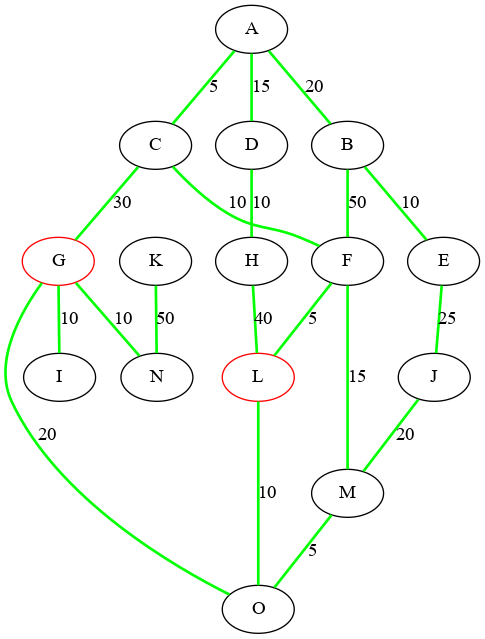
\includegraphics[width=0.5\textwidth]{img/graph_sim_test.png}
    \caption{Grafo Teste da Simulação}
    \label{fig:graph_sim_test}
\end{figure}

\clearpage
\loadgeometry{default}

\section{Implementação do Problema}

\subsection{Classes Implementadas}
Para a implementação do problema, foram criadas os seguintes módulos:

\begin{itemize}
    \item \texttt{algorithms/}
    \begin{itemize}
        \item \texttt{bfs:} Implementa o algoritmo de procura em largura;
        \item \texttt{dfs:} Implementa o algoritmo de procura em profundidade;
        \item \texttt{ucs:} Implementa o algoritmo de procura de custo uniforme;
        \item \texttt{astar:} Implementa o algoritmo A*;
        \item \texttt{greedy:} Implementa o algoritmo Gulosa.
    \end{itemize}
    \item \texttt{graph/}
    \begin{itemize}
        \item \texttt{graph:} Representa um grafo com atributos como nós, arestas, custos e valores 
        heurísticos;
        \item \texttt{node:} Representa um nó no grafo, e os seus dados, como nome, combustível,
        catástrofe, veículos e suprimentos;
        \item \texttt{heuristics:} Implementa três diferentes heurísticas para os algoritmos de 
        procura A* e Gulosa, que são usadas para calcular os valores heurísticos dos nodos;
    \end{itemize}

    \item \texttt{catastrophe:} Armazena informações sobre uma catástrofe, como tempo de resposta
    e demanda de suprimentos;

    \item \texttt{vehicle:} Modela veículos com atributos como nome, categoria, velocidade,
    capacidade de carga e métodos para gerenciar combustível e carga;

    \item \texttt{supply:} Armazena informações sobre um suprimento, como tipo, quantidade e tempo
    de perecibilidade;

    \item \texttt{mission\_planner:} É responsável por planear a missão. Chama os algoritmos de procura
    e retorna o melhor caminho para cada veículo, considerando os suprimentos e catástrofes no ambiente.
    Armazena o grafo, a frota de veículos, as catástrofes e os suprimentos;

    \item \texttt{operation:} Representa o conjunto de operações \textit{start}, \textit{move}, \textit{load},
    \textit{drop} e \textit{refuel} dos veículos, e onde acontecem;

    \item \texttt{simulation\_data:} Inicializa a simulação criando catástrofes e veículos,
    e inciliazando o \texttt{Mission Planner}. É usada para definir os dados iniciais dos quais, grafo, veículos,
    suprimentos e nodos de catástrofes, bem como a definição de função de heurística a ser utilizada e
    nodos e arestas destrutíveis;

    \item \texttt{main:} Módulo principal que gere a execução do programa, e interage com o utilizador
    através de menus.
\end{itemize}


\subsection{Operadores Implementados}

Foram implementados os seguintes operadores para simular as ações possíveis:

\begin{itemize}
    \item \texttt{Start:} Indica o nodo onde o veículo começa a sua missão (somente usado para 
    aprimoração do \textit{output});
    \item \texttt{Move:} Desloca o veículo entre localizações, considerando consumo 
    de combustível;
    \item \texttt{Load:} Carrega suprimentos no veículo, respeitando a capacidade de carga;
    \item \texttt{Drop:} Descarrega suprimentos do veículo;
    \item \texttt{Refuel:} Simula o tempo de reabastecimento (6 segundos por litro).
\end{itemize}

\clearpage

\subsection{Implementação de Restrições}

Os veículos começam a sua missão com o combustível cheio (de acordo com as capacidades correspondentes), e com a carga de suprimentos
vazia. Logo no primeiro nodo, são carregados suprimentos de acordo com a capacidade do veículo.

A cada movimentação, é diminuído o combustível disponível, até que o veículo necessite de reabastecimento, cujo tempo é
calculado com base na capacidade de combustível e no tempo de abastecimento de um litro: 6 segundos.

Os suprimentos também vão diminuindo à medida que são descarregados, e são reabastecidos
nos locais de abastecimento nos nodos (para conveniência, existe uma quantidade infinita de suprimentos, bem como combustível).

Também foram implementadas destruições de nodos, bem como de arestas, que representam o bloqueio de certos caminhos devido a desastres naturais.
Quando um nodo do grafo é destruído, o veículo que lá se encontra é dado como perdido e todas as arestas que o ligam a outros nodos
são removidas. Como supramencionado, a destruição de nodos e/ou arestas são definidas no ficheiro \texttt{simulation\_data.py}.
Os algoritmos de procura não têm conhecimento atempado dessas condições de destruição, sendo assim, o programa responsável por
se adaptar dinamicamente a essas condições.

O grau de urgência de uma catástrofe é dado pelo tempo de chegada e o seu tempo de resposta máximo.

\section{Algoritmos de Procura Utilizados}

Para a resolução do problema, foram utilizados os seguintes algoritmos de procura:

\begin{itemize}
    \item \textbf{\textit{Breadth-First Search (BFS):}} Procura em Largura, que expande todos os nós de um nível antes de passar para o próximo.
    \item \textbf{\textit{Depth-First Search (DFS):}} Procura em Profundidade, que expande um nó até ao limite antes de retroceder.
    \item \textbf{\textit{Uniform-Cost Search (UCS):}} Procura de Custo Uniforme, que expande o nó com menor custo de caminho.
    \item \textbf{\textit{A* Search:}} Procura A*, que combina a procura gulosa com a procura de custo uniforme, utilizando o valor heurístico.
    \item \textbf{\textit{Greedy:}} Procura Gulosa, que expande o nó que parece mais promissor, com no valor heurístico.
\end{itemize}

\section{Heurísticas Desenvolvidas}

Para os algoritmos A* e Gulosa, foram criadas as seguintes heurísticas:

\begin{itemize}
    \item \textbf{Distância:} Distâncias para cada catástrofe por tipo de veículo e nível de acesso;
    \item \textbf{Tempo, Distância e Combustível:} Prioridades para cada catástrofe por tipo de veículo, nível de acesso,
    tempo de chegada do veículo - tempo de resposta na catástrofe e combustível: 
    \texttt{distance + time\_arrival\_vehicle - \\ catastrophe\_response\_time + fuel};
    \item \textbf{Tempo, Distância, Combustível e Carga:} Prioridades para cada catástrofe por tipo de veículo, nível de acesso,
    tempon de chegada do veículo - tempo de resposta na catastrofe, carga do veículo/demanda da catastrofe e combustível: 
    \texttt{distance + time\_arrival\_vehicle - catastrophe\_response\_time + fuel + cargo}.
\end{itemize}

A distância é calculada com recurso ao algoritmo de Dijkstra (Custo Uniforme), que calcula o caminho mais curto entre dois nodos, para cada tipo de veículo.

Esta decisão permitiu a utilização de uma heurística mais precisa, e consequentemente com melhores resultados, sendo esta mais precisa que por exemplo a distância Euclidiana ou
a distância de Manhattan.

O cálculo dos valores heurísticos é realizado na inicialização do \texttt{Mission Planner}, ou quando o utilizador escolhe outra heurística a utilizar,
em vez de iterativamente nos algoritmos de pesquisa, devido ao cálculo da distância ser custoso computacionalmente.

\clearpage

\section{Estratégias para a Resolução do Problema}

Um dos maiores desafios deste projeto foi garantir que os veículos são utilizados de forma conjunta, de forma a otimizar a distribuição dos suprimentos.
Para tal, começou-se por definir quais dos veículos conseguem aceder as diferentes catástrofes do grafo a tempo, utilizando o algoritmo de pesquisa escolhido
pelo utilizador. 

Com estes dados, foi desenvolvida uma função que permite, para cada catástrofe, a escolha do veículo mais adequado para a sua resolução,
baseado no número de veículos que conseguem aceder a essa catástrofe, o consumo de combustível e a capacidade de carga do veículo.

Na primeira estrutura de dados, é também guardado o conjunto de operações calculadas pelo algoritmo para o veículo no auxílio da catástrofe, de forma 
a não ser necessário recalcular essas operações.

Quando o nodo ou uma aresta são destruídos, a estrutura de dados é recriada, assim como os veículos são revinculados às catástrofes que conseguem aceder. 

%===============================================================================
% END TAREFAS REALIZADAS E DECISÕES TOMADAS
%===============================================================================

%===============================================================================
% BEGIN DISCUSSÃO DOS RESULTADOS OBTIDOS
%===============================================================================

\chapter{Discussão dos Resultados Obtidos}

\section{Resultados com BFS}

Utilizando o algoritmo \textit{Breadth-First Search}, foi possível obter os seguintes resultados:


\textbf{Tempo de Resposta:} \\
O tempo de resposta foi de 575 segundos para a simulação de uma cidade média, 288 segundos para a simulação
do arquipélago dos Açores, e 38 segundos para a simulação de teste. \\

\textbf{Combustível Utilizado:} \\
O combustível utilizado foi de 36,6 litros para a simulação de uma cidade média, 382,61 litros para a simulação
do arquipélago dos Açores, e 9 litros para a simulação de teste. \\

\clearpage

\textbf{Caminho Percorrido:} \\
O caminho percorrido foi o seguinte:
\begin{itemize}
    \item \textbf{Cidade Média:}
        \begin{itemize}
            \item Mota: $A \rightarrow C \rightarrow F \rightarrow I \rightarrow J \rightarrow I
             \rightarrow J \rightarrow I \rightarrow J \rightarrow I \rightarrow J \rightarrow I$ \\
            \item Carro: $A \rightarrow C \rightarrow F \rightarrow E \rightarrow F$ \\
            \item Drone: $A \rightarrow B \rightarrow A$ (várias vezes)
        \end{itemize}
    \item \textbf{Açores:}
        \begin{itemize}
            \item Avião: $Graciosa \rightarrow Sao Jorge \rightarrow Pico \rightarrow Faial$ \\
            \item Helicóptero: $Graciosa \rightarrow Terceira \rightarrow Pico$ \\
            \item Barco: $Terceira \rightarrow Santa Maria$ \\
            \item Barco2: $Terceira \rightarrow Sao Miguel$
        \end{itemize}
    \item \textbf{Teste:}
        \begin{itemize}
            \item Mota: $A \rightarrow C \rightarrow G \rightarrow N \rightarrow G$ \\
            \item Carro: $A \rightarrow B \rightarrow F \rightarrow L$
        \end{itemize}
\end{itemize}

\clearpage

\section{Resultados com DFS}

Utilizando o algoritmo \textit{Depth-First Search}, foi possível obter os seguintes resultados:

\textbf{Tempo de Resposta:} \\
O tempo de resposta foi de 575 segundos para a simulação de uma cidade média, 288 segundos para a simulação
do arquipélago dos Açores, e 68 segundos para a simulação de teste.

\textbf{Combustível Utilizado:} \\
O combustível utilizado foi de 37.2 litros para a simulação de uma cidade média, 311.91 litros para a simulação
do arquipélago dos Açores, e 10.61 litros para a simulação de teste.

\clearpage

\textbf{Caminho Percorrido:} \\
O caminho percorrido foi o seguinte:
\begin{itemize}
    \item \textbf{Cidade Média:}
        \begin{itemize}
            \item Mota: $A \rightarrow E \rightarrow H \rightarrow J \rightarrow I \rightarrow J
             \rightarrow I \rightarrow J \rightarrow I \rightarrow J \rightarrow I \rightarrow J \rightarrow I$ \\
            \item Carro: $A \rightarrow C \rightarrow F \rightarrow E \rightarrow F$ \\
            \item Drone: $A \rightarrow B \rightarrow A$ (várias vezes)
        \end{itemize}
    \item \textbf{Açores:}
        \begin{itemize}
            \item Avião: $Graciosa \rightarrow Sao Jorge \rightarrow Pico \rightarrow Faial$ \\
            \item Helicóptero: $Graciosa \rightarrow Sao Jorge \rightarrow Pico$ \\
            \item Barco: $Terceira \rightarrow Santa Maria$ \\
            \item Barco2: $Terceira \rightarrow Sao Miguel$
        \end{itemize}
    \item \textbf{Teste:}
        \begin{itemize}
            \item Mota: $A \rightarrow D \rightarrow H \rightarrow L \rightarrow O
            \rightarrow G \rightarrow N \rightarrow G \rightarrow N \rightarrow G$ \\
            \item Carro: $A \rightarrow D \rightarrow H \rightarrow L$
        \end{itemize}
\end{itemize}

\clearpage

\section{Resultados com Uniforme}

Utilizando o algoritmo \textit{Uniform-Cost Search}, foi possível obter os seguintes resultados:

\textbf{Tempo de Resposta:} \\
O tempo de resposta foi de 575 segundos para a simulação de uma cidade média, 288 segundos para a simulação
do arquipélago dos Açores, e 38 segundos para a simulação de teste. \\

\textbf{Combustível Utilizado:} \\
O combustível utilizado foi de 36.6 litros para a simulação de uma cidade média, 382.61 litros para a simulação
do arquipélago dos Açores, e 8.2 litros para a simulação de teste. \\

\clearpage

\textbf{Caminho Percorrido:} \\
O caminho percorrido foi o seguinte:
\begin{itemize}
    \item \textbf{Cidade Média:}
        \begin{itemize}
            \item Mota: $A \rightarrow C \rightarrow F \rightarrow I \rightarrow J \rightarrow I
             \rightarrow J \rightarrow I \rightarrow J \rightarrow I \rightarrow J \rightarrow I$ \\
            \item Carro: $A \rightarrow C \rightarrow F \rightarrow E \rightarrow F$ \\
            \item Drone: $A \rightarrow B \rightarrow A$ (várias vezes)
        \end{itemize}
    \item \textbf{Açores:}
        \begin{itemize}
            \item Avião: $Graciosa \rightarrow Sao Jorge \rightarrow Faial$ \\
            \item Helicóptero: $Graciosa \rightarrow Terceira \rightarrow Pico$ \\
            \item Barco: $Terceira \rightarrow Santa Maria$ \\
            \item Barco2: $Terceira \rightarrow Sao Miguel$
        \end{itemize}
    \item \textbf{Teste:}
        \begin{itemize}
            \item Mota: $A \rightarrow C \rightarrow G \rightarrow N \rightarrow G
            \rightarrow N \rightarrow G $ \\
            \item Carro: $A \rightarrow D \rightarrow H \rightarrow L$
        \end{itemize}
\end{itemize}

\clearpage

\section{Resultados com Gulosa}

Utilizando o algoritmo da Gulosa com a primeira heurística, foi possível obter os seguintes resultados:

\textbf{Tempo de Resposta:} \\
O tempo de resposta foi de 575 segundos para a simulação de uma cidade média, 288 segundos para a simulação
do arquipélago dos Açores, e 38 segundos para a simulação de teste. \\

\textbf{Combustível Utilizado:} \\
O combustível utilizado foi de 35,8 litros para a simulação de uma cidade média, 311,91 litros para a simulação
do arquipélago dos Açores, e 4,6 litros para a simulação de teste. \\

\clearpage

\textbf{Caminho Percorrido:} \\
O caminho percorrido foi o seguinte:
\begin{itemize}
    \item \textbf{Cidade Média:}
        \begin{itemize}
            \item Mota: $A \rightarrow E \rightarrow F \rightarrow I \rightarrow J \rightarrow I
             \rightarrow J \rightarrow I \rightarrow J \rightarrow I \rightarrow J \rightarrow I$ \\
            \item Carro: $A \rightarrow C \rightarrow F \rightarrow E \rightarrow F$ \\
            \item Drone: $A \rightarrow B \rightarrow A$ (várias vezes)
        \end{itemize}
    \item \textbf{Açores:}
        \begin{itemize}
            \item Avião: $Graciosa \rightarrow Sao Jorge \rightarrow Faial$ \\
            \item Helicóptero: $Graciosa \rightarrow Sao Jorge \rightarrow Pico$ \\
            \item Barco: $Terceira \rightarrow Santa Maria$ \\
            \item Barco2: $Terceira \rightarrow Sao Miguel$
        \end{itemize}
    \item \textbf{Teste:}
        \begin{itemize}
            \item Mota: $A \rightarrow C \rightarrow G \rightarrow N \rightarrow G
            \rightarrow N \rightarrow G$ \\
            \item Carro: $A \rightarrow C \rightarrow F \rightarrow L$
        \end{itemize}
\end{itemize}

\clearpage

\section{Resultados com A*}

Utilizando o algoritmo A* com a primeira heurística, foi possível obter os seguintes resultados:

\textbf{Tempo de Resposta:} \\
O tempo de resposta foi de 575 segundos para a simulação de uma cidade média, 288 segundos para a simulação
do arquipélago dos Açores, e 38 segundos para a simulação de teste. \\

\textbf{Combustível Utilizado:} \\
O combustível utilizado foi de 36,4 litros para a simulação de uma cidade média, 311,91 litros para a simulação
do arquipélago dos Açores, e 4,6 litros para a simulação de teste. \\

\clearpage

\textbf{Caminho Percorrido:} \\
O caminho percorrido foi o seguinte:
\begin{itemize}
    \item \textbf{Cidade Média:}
        \begin{itemize}
            \item Mota: $A \rightarrow E \rightarrow F \rightarrow I \rightarrow J \rightarrow I
             \rightarrow J \rightarrow I \rightarrow J \rightarrow I \rightarrow J \rightarrow I$ \\
            \item Carro: $A \rightarrow C \rightarrow F \rightarrow E \rightarrow F$ \\
            \item Drone: $A \rightarrow B \rightarrow A$ (várias vezes)
        \end{itemize}
    \item \textbf{Açores:}
        \begin{itemize}
            \item Avião: $Graciosa \rightarrow Sao Jorge \rightarrow Faial$ \\
            \item Helicóptero: $Graciosa \rightarrow Sao Jorge \rightarrow Pico$ \\
            \item Barco: $Terceira \rightarrow Santa Maria$ \\
            \item Barco2: $Terceira \rightarrow Sao Miguel$
        \end{itemize}
    \item \textbf{Teste:}
        \begin{itemize}
            \item Mota: $A \rightarrow C \rightarrow G \rightarrow N \rightarrow G
            \rightarrow N \rightarrow G$ \\
            \item Carro: $A \rightarrow C \rightarrow F \rightarrow L$
        \end{itemize}
\end{itemize}

\clearpage

\section{Análise dos Resultados}

Os resultados mostram que, entre os algoritmos de procura informada, A* e Gulosa apresentaram desempenhos muito semelhantes no consumo de combustível, graças ao uso de uma heurística completa. Esta característica permitiu que ambos orientassem eficientemente a procura, resultando em trajetos otimizados e diferenças mínimas entre os dois métodos.

Nos algoritmos de procura cega, o UCS destacou-se por obter trajetos mais eficientes em termos de consumo de combustível quando comparado com BFS e DFS. Este desempenho superior deve-se ao facto de o UCS considerar os custos acumulados ao longo do caminho, enquanto BFS e DFS apenas seguem critérios de ordem ou profundidade, sem avaliar os custos das ações.

Em termos de tempos de resposta, não foram observadas diferenças significativas entre os algoritmos, sugerindo que a complexidade intrínseca dos cenários testados foi o principal fator de variação.

Conclui-se que, enquanto os métodos informados beneficiaram diretamente da heurística completa, o UCS revelou-se a opção mais robusta entre os algoritmos cegos, destacando-se pelo equilíbrio entre simplicidade e eficiência no consumo de recursos.

%===============================================================================
% END DISCUSSÃO DOS RESULTADOS OBTIDOS
%===============================================================================

%===============================================================================
% BEGIN CONCLUSÃO E TRABALHO FUTURO
%===============================================================================
\chapter{Conclusão e Trabalho Futuro}

\section{Conclusão}

O trabalho realizado demonstra de forma clara a eficácia dos algoritmos de procura em resolver problemas logísticos complexos
em cenários de emergência. Destaca-se a superioridade do algoritmo A* e do UCS, em diferentes contextos, no equilíbrio entre eficiência
de recursos e tempo de resposta. Além disso, a utilização de heurísticas completas evidenciou a importância de critérios bem definidos
na melhoria de resultados. 

\section{Trabalho Futuro}
A nível de trabalho futuro, destacam-se as seguintes áreas:

\begin{itemize}
    \item {\textbf{Perecibilidade dos Alimentos:}} Implementar um modelo mais realista para a perecibilidade dos alimentos, considerando
    que, a partir do momento em que os suprimentos são abastecidos no veículo, o tempo de deterioração começa a contar. Isto seria efetuado
    através de um contador de tempo que simula a deterioração dos alimentos, e que seria considerado na escolha de rotas e prioridades.

    \item{\textbf{Reutilização de Veículos noutras Operações:}} Implementar a capacidade do veículo, após ter completado as suas operações,
    procurar outras zonas afetadas em que o veículo que está a ajudar ainda não tenha, nem vá completar, ou zonas afetadas sem quaisquer veículos a ajudar.
    Deste modo, este veículo poderia ser reutilizado nessa catástrofe, completando-a mais rapidamente. 
    Tal seria implementado pelo registo dos veículos atribuídos a uma catástrofe, e, no fim de um veículo completar as suas operações, procurar
    primeiramente, por catástrofes sem veículos atribuídos, ou catástrofes com veículos atribuídos, mas que não vão completar a tempo.
\end{itemize}

%===============================================================================
% END CONCLUSÃO E TRABALHO FUTURO
%===============================================================================

%===============================================================================
% BEGIN REFERÊNCIAS
%===============================================================================

%% Change bibliography name from “Bibliografia” to “Referências”
\renewcommand\bibname{Referências}

\begin{thebibliography}{9}

\bibitem{RussellNorvig}
Russell, S., \& Norvig, P. (2009). \textit{Artificial Intelligence - A Modern Approach} (3rd ed.). Pearson Education. ISBN-13: 9780136042594.

\bibitem{CostaSimoes}
Costa, E., \& Simões, A. (2008). \textit{Inteligência Artificial - Fundamentos e Aplicações}. FCA. ISBN: 978-972-722-34.

\end{thebibliography}

%% Add bibliografia to index
\addcontentsline{toc}{chapter}{Referências}

%===============================================================================
% END REFERÊNCIAS
%===============================================================================

\end{document}
